\documentclass[13pt,a4paper]{article}

\usepackage[utf8]{inputenc}
\usepackage[MeX]{polski}
\usepackage{graphicx}
\usepackage{wrapfig}
\usepackage{color}
\usepackage{amsmath}
\usepackage{amssymb}
\usepackage[inkscapelatex=false]{svg}
\usepackage{array, makecell}
\usepackage{mhchem}
\usepackage{tabularx}
\usepackage{svg}
\usepackage{braket}

\usepackage{multicol}
\usepackage{colortbl}
\usepackage[Export]{adjustbox}
\adjustboxset{max size={0.9\linewidth}{0.9\paperheight}}
\usepackage[colorlinks=true,linkcolor=red,citecolor=green]{hyperref}

\textwidth=16cm
\textheight=23cm
\topmargin=-2cm
\oddsidemargin=0cm
\setlength{\parindent}{0em}
\setlength{\parskip}{0.6em}
\setlength{\jot}{12pt}
\renewcommand{\arraystretch}{1.4}
\renewcommand{\theadfont}{\bfseries}
\newcommand{\todo}[1]{\textcolor{red}{TODO: #1}}


\begin{document}
\title{
    \LARGE
    \textbf{Praca domowa nr 1}
}
\author{
    \large
    Dawid Karpiński, 8.03.2024 r.
}
\date{}
\maketitle

\section{Histogram N(x)}

Poniżej zamieszczono histogram liczby konfliktów $N(x)$, o liczbie ofiar w jednorodnych przedziałach wartości (binach).

Jako szerokość pojedynczego binu przyjęto $\Delta{x}=1000$.

\begin{figure}[ht!]
    \centering
    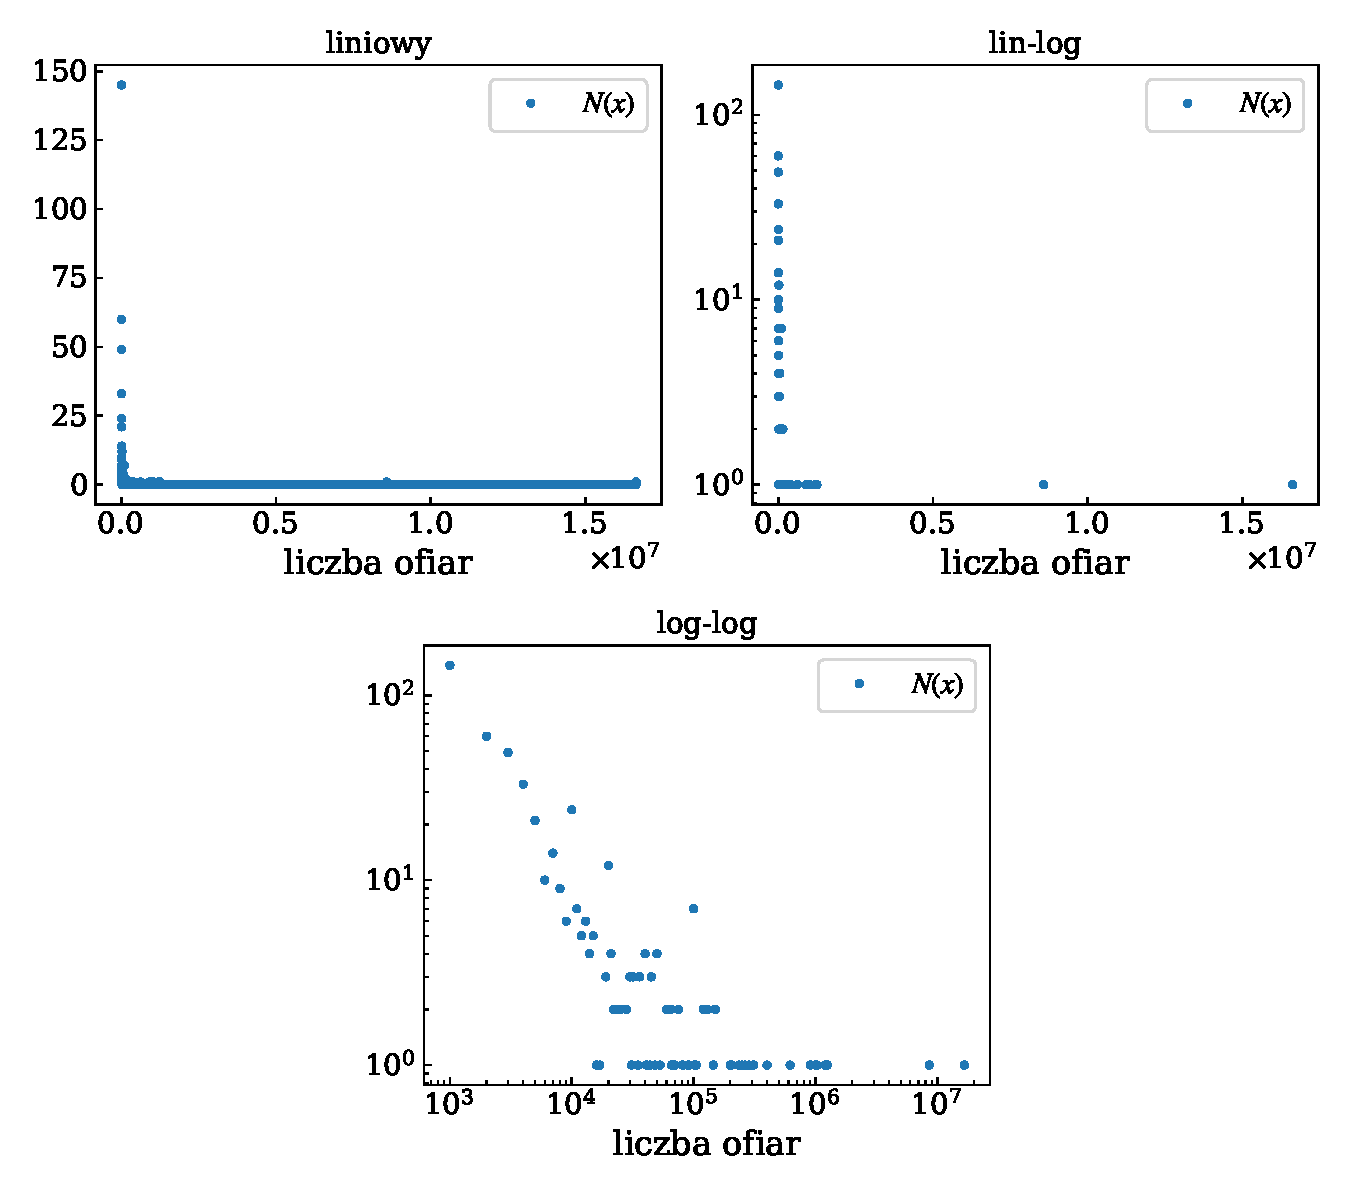
\includegraphics{./hist.pdf}
\end{figure}

Można stwierdzić, że najbardziej czytelne są dane przedstawione na wykresie w skali log-log.


\section{Prawdopodobieństwo P(x)}

Następnie przygotowano wykres prawdopodobieństwa, licząc je jako:

$$
P(x) = \frac{N(x)}{N\Delta{x}}.
$$

\begin{figure}[ht!]
    \centering
    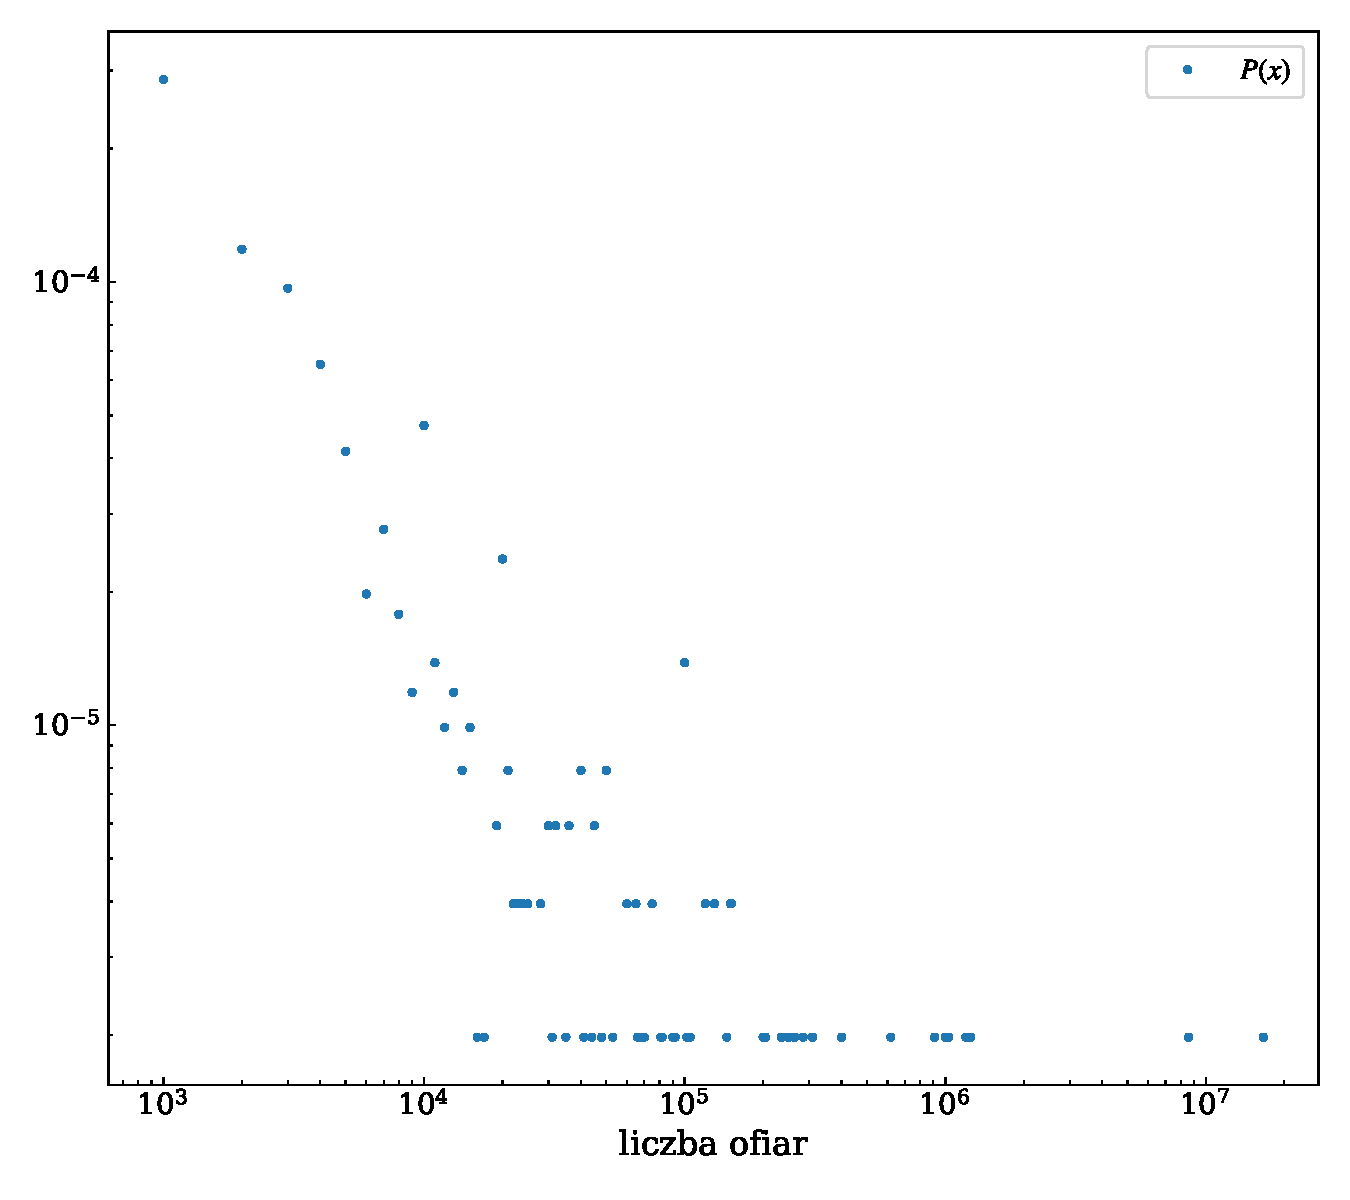
\includegraphics{./hist_prob.pdf}
\end{figure}

Każdy punkt przedstawia prawdopodobieństwo wystąpienia konfliktu w danym przedziale ofiar. Dlatego należy podzielić przez szerokość binu.


\pagebreak
\section{Histogram logarytmiczny}

Dane konfliktów i ofiar były bardzo rzadko rozmieszczone, dlatego sporządzono histogram logarytmiczny. Szerekość każdego kolejnego binu wzrasta potęgowo, w tym przypadku wybrano jako podstawę $a=2$.

Zatem, biny mają wartości: $(x_0, 2x_0), (2x_0, 2^2x_0), ...$, gdzie $x_0$ to najmniejsza wartość ofiar spośród dostępnych danych.

\begin{figure}[ht!]
    \centering
    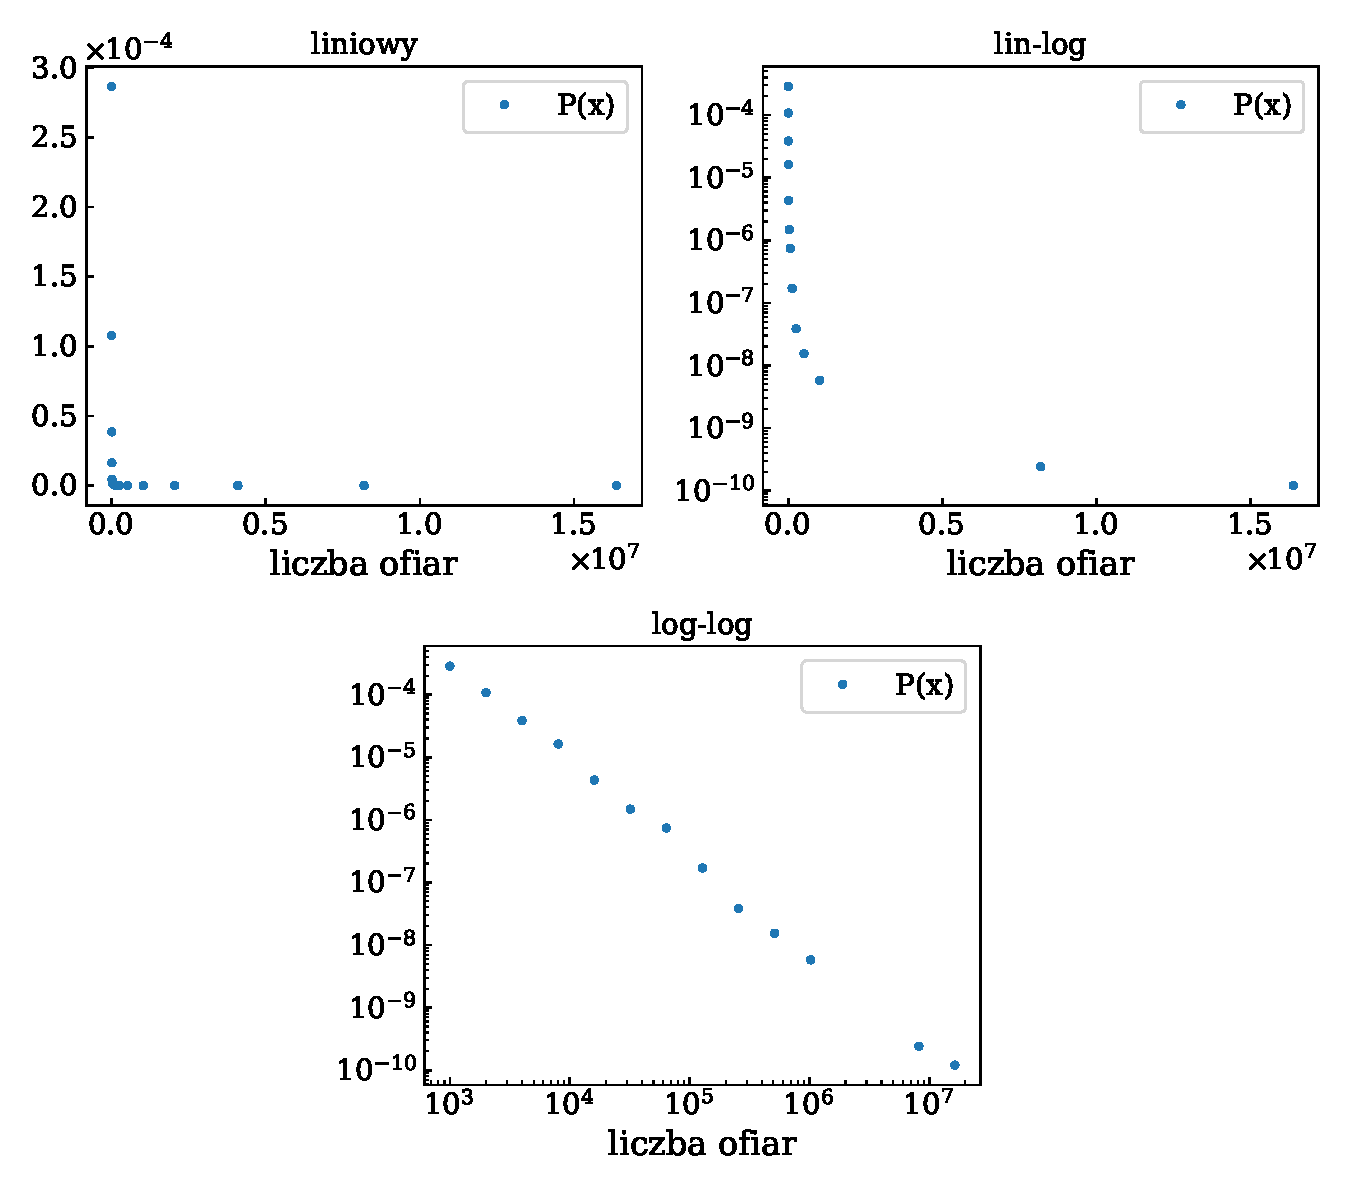
\includegraphics{./hist_log.pdf}
\end{figure}

W skali log-log, punkty układają się w linię prostą, co sugeruje rozkład potęgowy danych.


\pagebreak
\section{Skumulowany rozkład $P^c(x)$}

Podobnie jak w przypadku histogramu logarytmicznego, rozkład skumulowany w skali log-log również wykazuje własności rozkładu potęgowego.

\begin{figure}[ht!]
    \centering
    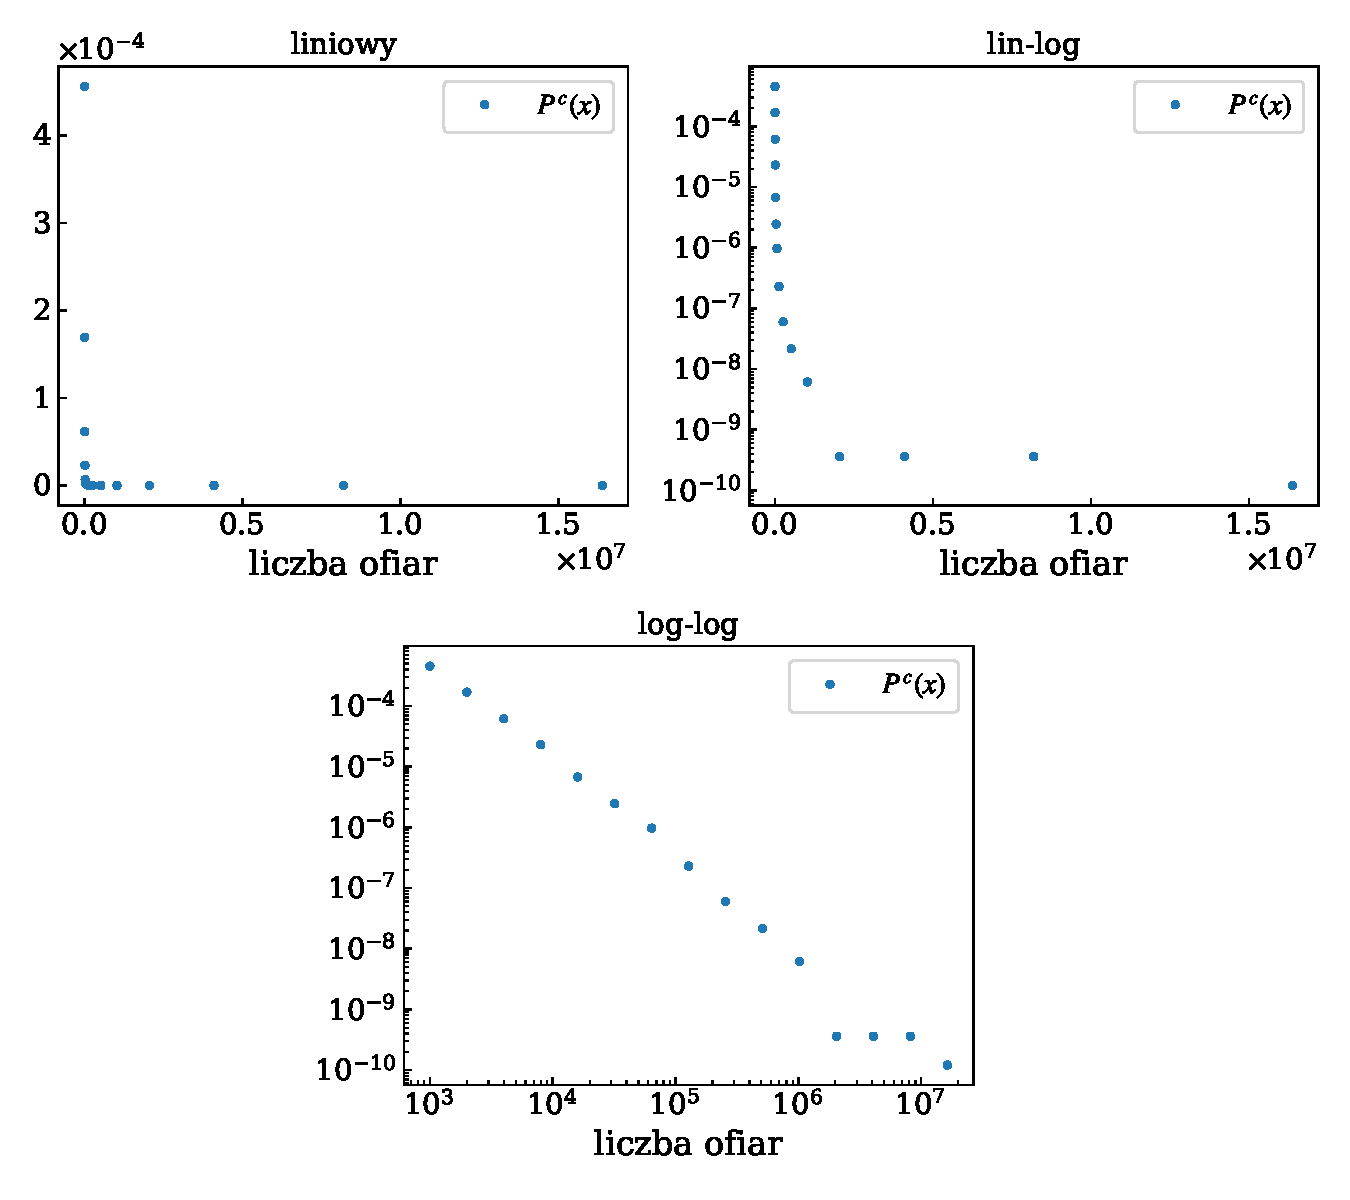
\includegraphics{./hist_cum.pdf}
\end{figure}

Ponadto, w skali log-log w granicach liczby ofiar $10^6-10^7$ widać mało zmieniające się wartości, co pokazuje dużą różnicę i dotklilwość tych konfliktów, w porównaniu do reszty.

\end{document}
